% Instructions to change to html version:
% Comment out:
%  minipage, multicols,columnbreak, mathbf, hrule
% Replace all: \begin{minipage}% %%\end{minipage} %%%\begin{mulicols}  %%%\end{mulicols}  %%\columnbreak % %%\begin{framed} %%%\end{framed} %%%\hrule
% Search for \mathbf \mathcal
% Replace \\] with \[ and \) with \(
% Enclose graphics in figure environments and add captions
% Re-tag \df environments as sections, subsections, etc.
% Command Line Code to Create html version:
%First: pdflatex -shell-escape filename.tex                                   
%Second, for each figure: inkscape "filename-figure1.pdf" -o "filename-figure1.png"
% Third: htlatex filename.tex "ht5mjlatex.cfg, charset=utf-8" " -cunihtf -utf8"


\documentclass[10pt]{article}

%\usepackage{tikz, pgf,pgfplots,wasysym,array}
%\usepackage{wasysym,array}

\usepackage{amsmath,amssymb}

\ifdefined\HCode
  \def\pgfsysdriver{pgfsys-tex4ht-updated.def}
\fi 
%\ifdefined\HCode
%  \def\pgfsysdriver{pgfsys-dvisvgm4ht.def}
%\fi 
\usepackage{tikz}
\usetikzlibrary{calc,decorations.markings,arrows}
\usepackage{pgfplots}

\pgfplotsset{compat=1.12}
\usepackage{myexternalize}
\usetikzlibrary{calc,decorations.markings,arrows}
\usepackage{framed}
\usepackage[none]{hyphenat}

\input{../../../common/1336_header_test.tex}

\begin{document}

\renewcommand{\myTitle}{MATH 2330: Multivariable Calculus}

\renewcommand{\mySubTitle}{Section 5.1: Double Integrals over Rectangular Regions}
%~\hfill Name: \underline{~~~~~~~~~~~~~~~~~~~~~~~~~~~~~~~~~~~~~~~~~~~~~~~}

\lectTitle{\vspace*{-.5in}\myTitle}{\vspace*{.1in}\mySubTitle \vspace*{-.25in}}



%\hspace*{-.8in}%\begin{minipage}{1.25\textwidth}
%\begin{framed}

\section*{Double Integral Definition:}




%\begin{multicols}{2}

\begin{figure}[!hbtp]
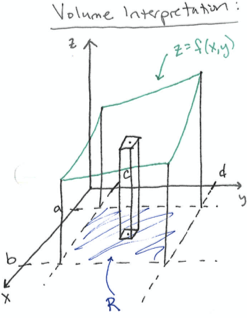
\includegraphics[height=2in]{Ch12s1-Volume1.png}
\hspace*{1in}
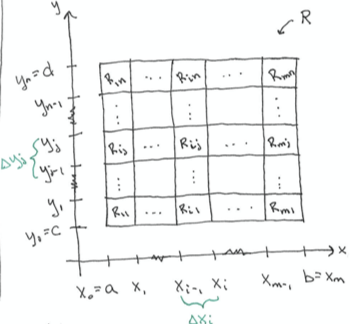
\includegraphics[height=2in]{Ch12s1-Rectangle1.png}
\caption{Double Integral Definition Diagrams}
\end{figure}

%\columnbreak


A  \textbf{double integral over a rectangle} \(R:[a,b] \times [c,d]\) is defined as:
\[
\iint_R f(x,y)\ dA = \lim_{\text{max} \Delta x_i, \Delta y_j \rightarrow 0}
 \sum_{i=0}^m \sum_{j=0}^n f\left( x_{ij}^*, y_{ij}^* \right) \Delta A_{ij}
\]

~\\
\textbf{Key Idea:}\\
\begin{itemize}
\item Split the rectangle into \(mn\) sub-rectangles of area\\ \(\Delta A_{ij} = \Delta x_i \Delta y_j\)
\item Pick a sample point from each sub-rectangle: \(\left( x_{ij}^*, y_{ij}^* \right) \)
\item Evaluate the function at each sample point: \(f\left( x_{ij}^*, y_{ij}^* \right)\)
\item Calculate the volume of a column: \(V_{ij} =  f\left( x_{ij}^*, y_{ij}^* \right) \Delta A_{ij}\)
\item Add up the volumes of the columns to estimate the total volume: \(V \approx V_{11} + V_{12} + \ldots + V_{mn}\) 
\end{itemize}


%\end{multicols}

%\hrule
\vspace*{.2in}

\section*{Fubini's Theorem:}
If \(f(x,y)\) is continuous on \(R=\{ (x,y) | a\leq x \leq b, c\leq y \leq d\}\) then:
\[
\iint_R f(x,y)\ dA = \int_c^d \int_a^b f(x,y)\ dx\ dy =  \int_a^b\int_c^d f(x,y)\ dy\ dx
\]

\textbf{Key Ideas:}
\begin{itemize}
\item Order of Operations: work from the inside out (like parentheses!)
\item We can swap the order of integration in the iterated integrals
\item The final result should be a number, no \(x\)'s or \(y\)'s should remain
\item \underline{Partial Integration:}
\begin{itemize}
\item \(\int_a^b f(x,y)\ dx\): hold \(y\) fixed and integrate wrt \(x\).
\item \(\int_c^d f(x,y)\ dy\): hold \(x\) fixed and integrate wrt \(y\).
\end{itemize}
\end{itemize}

%\end{framed}

%\end{minipage}

%\begin{framed}
\section*{Partial Integration - Visual POV:}
\begin{figure}[hbtp]
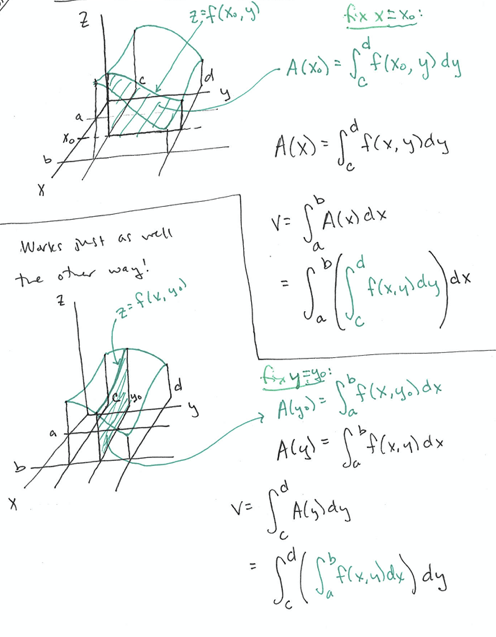
\includegraphics[height=.5\textheight]{Ch12s1-Slicing.png}
\caption{Partial Integration - Visual POV Diagrams}
\end{figure}


%\end{framed}

\section*{Examples:}


\begin{enumerate}[{Example} 1: ]

\addtocounter{enumi}{-1}

\item Evaluate \(\qquad \displaystyle \iint_{R} 3+4x \ dA, \qquad \qquad R= [0,1] \times [0,2]\)

\vfill

\item Evaluate \(\qquad \displaystyle \iint_{R} x^3 + y^5 \ dA, \qquad \qquad R= [-2,2] \times [0,2]\)


\vfill

\item Evaluate \(\qquad \displaystyle \int_0^1 \int_{\frac{1}{2}}^2 y e^{xy}\ dy\ dx\)

\vfill

\item Evaluate \(\qquad \displaystyle \iint_{R} \frac{\ln y}{xy} \ dA, \qquad \qquad R= [1,3] \times [1,5]\)

\vfill

\item Evaluate \(\qquad \displaystyle \iint_{R} \sqrt{1-y^2}\ dA, \qquad \qquad R= [0,2] \times [-1,1]\)

\vfill

\item True or False: \(\qquad \displaystyle \iint_{R} \cos\left(2\pi(y^2+x)\right) \ dA=0, \qquad \qquad R= [0,1] \times [0,1]\)


\end{enumerate}

\end{document}

